\documentclass[10pt,twocolumn,letterpaper]{article}

\usepackage{cvpr}
\usepackage{times}
\usepackage{epsfig}
\usepackage{graphicx}
\usepackage{amsmath}
\usepackage{amssymb}

% Include other packages here, before hyperref.

% If you comment hyperref and then uncomment it, you should delete
% egpaper.aux before re-running latex.  (Or just hit 'q' on the first latex
% run, let it finish, and you should be clear).
\usepackage[breaklinks=true,bookmarks=false]{hyperref}

\cvprfinalcopy % *** Uncomment this line for the final submission

\def\cvprPaperID{****} % *** Enter the CVPR Paper ID here
\def\httilde{\mbox{\tt\raisebox{-.5ex}{\symbol{126}}}}

% Pages are numbered in submission mode, and unnumbered in camera-ready
%\ifcvprfinal\pagestyle{empty}\fi
\setcounter{page}{1}
\begin{document}

%%%%%%%%% TITLE
\title{Deep Network Defined Error Correcting Code}

\author{Gan Tu\\
UC Berkeley\\
{\tt\small tugan@berkeley.edu}
}

\maketitle
%\thispagestyle{empty}

%%%%%%%%% ABSTRACT
\begin{abstract}
   Modern error correcting codes are used in wireless radio communications in order to detect and recover corrupted bits sent over noisy channels. Viterbi algorithm has been the popular decoding algorithm used for such purposes for its optimality. However, many of the algorithms used for radio nowadays depend on predefined scheme such as Trellis and generator matrices. In the research this semester, I explored the possibility of a deep neural network based approach to error correction, as an initial effort towards the goal of a end-to-end radio communication scheme in future. Specifically, I will briefly recap what I did this semester, what I learned, and what I found interesting in this report. I will also demonstrate some initial results obtained for Convolutional Encoding error correction by Feed Forward Neural Networks, Convolutional Neural Networks, Long Short Term Memory Networks (LSTM), and Bidirectional-LSTMs, compared against baseline optimal Viterbi decoding algorithm.
\end{abstract}

%%%%%%%%% BODY TEXT
\section{Model Architecture}

Please follow the steps outlined below when submitting your manuscript to
the IEEE Computer Society Press.  This style guide now has several
important modifications (for example, you are no longer warned against the
use of sticky tape to attach your artwork to the paper), so all authors
should read this new version.

%-------------------------------------------------------------------------
\subsection{Feed Forward Neural Networks}

All manuscripts must be in English.

\subsection{Convolutional Neural Networks}

Please refer to the author guidelines on the CVPR 2018 web page for a
discussion of the policy on dual submissions.

\subsection{Long Short Term Memory Networks (LSTM)}
Papers, excluding the references section,
must be no longer than eight pages in length. The references section
will not be included in the page count, and there is no limit on the
length of the references section. For example, a paper of eight pages
with two pages of references would have a total length of 10 pages.
{\bf There will be no extra page charges for CVPR 2018.}

\subsection{Bidirectional LSTM}
Overlength papers will simply not be reviewed.  This includes papers
where the margins and formatting are deemed to have been significantly
altered from those laid down by this style guide.  Note that this
\LaTeX\ guide already sets figure captions and references in a smaller font.
The reason such papers will not be reviewed is that there is no provision for
supervised revisions of manuscripts.  The reviewing process cannot determine
the suitability of the paper for presentation in eight pages if it is
reviewed in eleven.  


%-------------------------------------------------------------------------
\section{Experiments}

List and number all bibliographical references in 9-point Times,
single-spaced, at the end of your paper. When referenced in the text,
enclose the citation number in square brackets, for
example.  Where appropriate, include the name(s) of
editors of referenced books.

\subsection{Training Data}
List and number all bibliographical references in 9-point Times,
single-spaced, at the end of your paper. When referenced in the text,
enclose the citation number in square brackets, for
example.  Where appropriate, include the name(s) of
editors of referenced books.

\subsection{Results}
List and number all bibliographical references in 9-point Times,
single-spaced, at the end of your paper. When referenced in the text,
enclose the citation number in square brackets, for
example.  Where appropriate, include the name(s) of
editors of referenced books.

\begin{figure}[t]
\begin{center}
\fbox{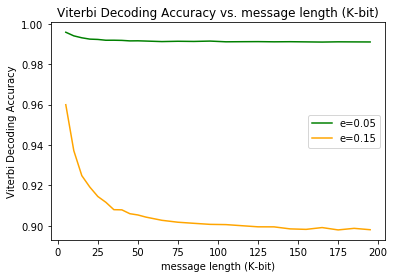
\includegraphics[width=0.8\linewidth]{img/viterbi.png}}
\end{center}
   \caption{Viterbi Accuracy over K-bit Message Length}
\end{figure}


\begin{figure}[t]
\begin{center}
\fbox{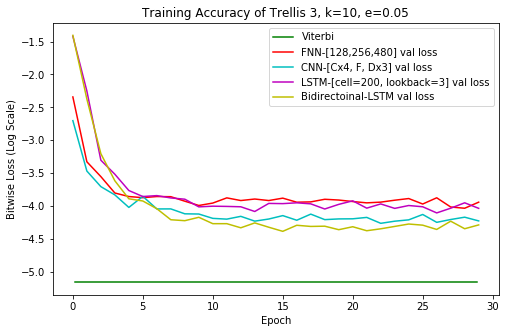
\includegraphics[width=0.8\linewidth]{img/k10-e05.png}}
\end{center}
   \caption{Short Message Length and Low Channel Corruption}
\end{figure}


\begin{figure}[t]
\begin{center}
\fbox{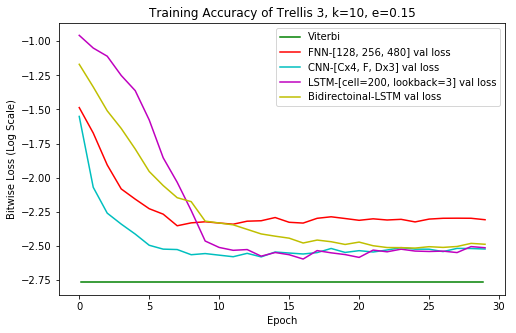
\includegraphics[width=0.8\linewidth]{img/k10-e15.png}}
\end{center}
   \caption{Short Message Length and High Channel Corruption}
\end{figure}


\begin{figure}[t]
\begin{center}
\fbox{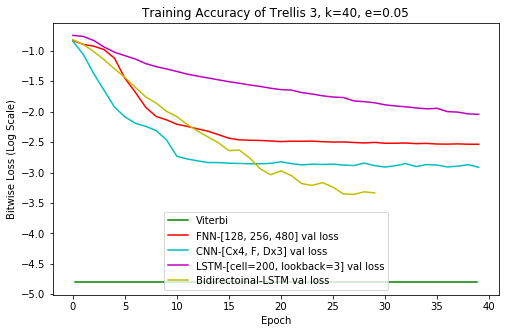
\includegraphics[width=0.8\linewidth]{img/k40-e05.png}}
\end{center}
   \caption{Long Message Length and Low Channel Corruption}
\end{figure}

\begin{table*}
\begin{center}
\begin{tabular}{|c|c|c|c|}
\hline
Architecture & Short Msg, Low Corruption & 
Short Msg, High Corruption & Long Msg, Low Corruption \\
\hline\hline
Viterbi Algorithm (Baseline) & 99.43 & 93.72 & 99.18  \\
\hline
Feed Forward Networks (FNN) & 98.17 & 90.14 & 92.06  \\
1D-CNN & \textbf{98.55} & \textbf{91.60} & 94.62\  \\
RNN-LSTM & 98.39 & 91.39 & 87.24  \\
Bidirectional LSTM & 98.45 & 91.34 & \textbf{96.46}  \\
\hline
\end{tabular}
\end{center}
\caption{Comparison of Test Accuracy over Top Performing Models (30 Epochs)}
\end{table*}


\subsection{Discussions}

List and number all bibliographical references in 9-point Times,
single-spaced, at the end of your paper. When referenced in the text,
enclose the citation number in square brackets, for
example.  Where appropriate, include the name(s) of
editors of referenced books.


\subsection{Next Step: New Architectures}

List and number all bibliographical references in 9-point Times,
single-spaced, at the end of your paper. When referenced in the text,
enclose the citation number in square brackets, for
example.  Where appropriate, include the name(s) of
editors of referenced books.

%-------------------------------------------------------------------------
\section{Semester Reflection}
List and number all bibliographical references in 9-point Times,
single-spaced, at the end of your paper. When referenced in the text,
enclose the citation number in square brackets, for
example.  Where appropriate, include the name(s) of
editors of referenced books.

\subsection{How I did}

List and number all bibliographical references in 9-point Times,
single-spaced, at the end of your paper. When referenced in the text,
enclose the citation number in square brackets, for
example.  Where appropriate, include the name(s) of
editors of referenced books.

\subsection{What I have learned}

List and number all bibliographical references in 9-point Times,
single-spaced, at the end of your paper. When referenced in the text,
enclose the citation number in square brackets, for
example.  Where appropriate, include the name(s) of
editors of referenced books.


%-------------------------------------------------------------------------

\medskip

\noindent
FAQ\medskip\\
{\bf Q:} Are acknowledgements OK?\\
{\bf A:} No.  Leave them for the final copy.\medskip\\
{\bf Q:} How do I cite my results reported in open challenges?
{\bf A:} To conform with the double blind review policy, you can report results of other challenge participants together with your results in your paper. For your results, however, you should not identify yourself and should not mention your participation in the challenge. Instead present your results referring to the method proposed in your paper and draw conclusions based on the experimental comparison to other results.\medskip\\

\end{document}
